\documentclass[a4paper,11pt]{article}
\usepackage[T1]{fontenc} % if needed
\usepackage{amssymb}
\usepackage{color}
\usepackage{xcolor}
\usepackage{amsmath}
\usepackage{tikz}
\usetikzlibrary{decorations.pathreplacing, decorations.markings, snakes}
\usetikzlibrary{arrows.meta}

\begin{document}

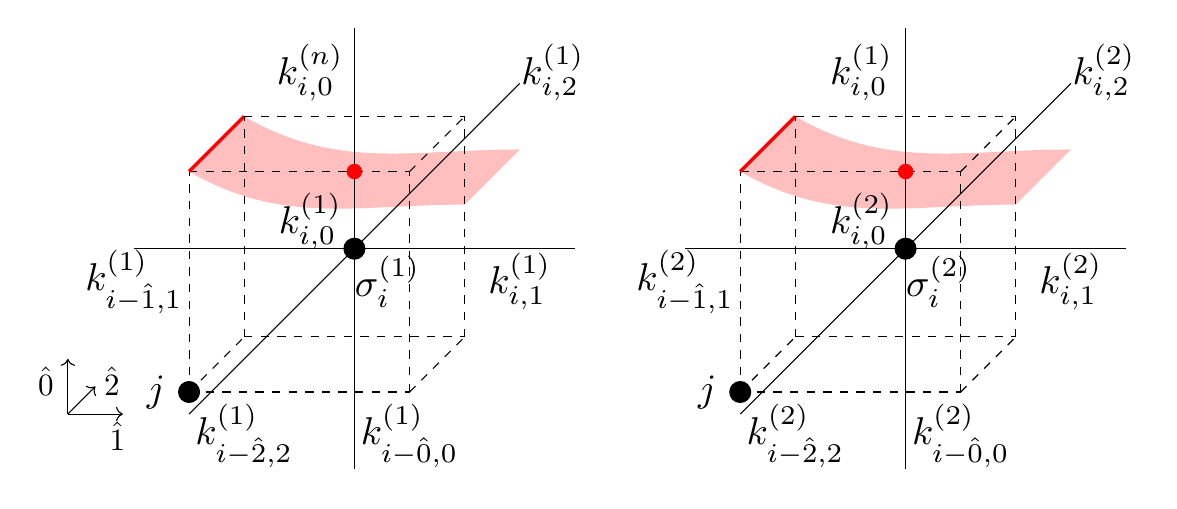
\begin{tikzpicture}[scale=1.4, every node/.style={scale=1.4}]
%
\fill[color=red!50!white, fill opacity=.5] (-1.5,.7) to[out=-30, in=180] (1,.4) -- (1.5,.9) to[out=180, in=-30] (-1,1.2) -- (-1.5,.7);
%
\draw (-1.5,-1.5)--(1.5,1.5);
\draw (-2,0)--(2,0);
\draw (0,-2)--(0,2);
%
\draw[dashed] (.5,-1.3)--(.5,.7); 
\draw[dashed] (-1.5,-1.3)--(.5,-1.3);
\draw[dashed] (-1.5,-1.3)--(-1.5,.7); 
\draw[dashed] (-1.5,.7)--(.5,.7);
%
\draw[dashed] (.5,-1.3)--(1,-.8);
\draw[dashed] (-1.5,-1.3)--(-1,-.8);
\draw[dashed] (.5,.7)--(1,1.2);
\draw[red,very thick] (-1.5,.7)--(-1,1.2);
%
\draw[dashed] (-1,-.8)--(1,-.8);
\draw[dashed] (-1,1.2)--(1,1.2);
\draw[dashed] (-1,-.8)--(-1,1.2);
\draw[dashed] (1,-.8)--(1,1.2);
%
\fill[color=black] (0,0) circle (.1);
\fill[color=black] (-1.5,-1.3) circle (.1);
\fill[color=red] (0,.7) circle (.07);
%
\draw (.3,-.3) node {$\sigma^{(1)}_i$};
\draw (-1.8,-1.3) node {$j$};
%
\draw (-1,-1.7) node {$k^{(1)}_{i-\hat{2},2}$};
\draw (1.8,1.6) node {$k^{(1)}_{i,2}$};
\draw (1.5,-.3) node {$k^{(1)}_{i,1}$};
\draw (-2,-.3) node {$k^{(1)}_{i-\hat{1},1}$};
\draw (.5,-1.7) node {$k^{(1)}_{i-\hat{0},0}$};
\draw (-.4,.25) node {$k^{(1)}_{i,0}$};
\draw (-.4,1.6) node {$k^{(n)}_{i,0}$};
%
\draw[->] (-2.2-.4,-1.5)--(-1.7-.4,-1.5);
\draw[->] (-2.2-.4,-1.5)--(-1.95-.4,-1.25);
\draw[->] (-2.2-.4,-1.5)--(-2.2-.4,-1);
\draw (-2.4-.4,-1.2) node[scale = .8] {$\hat{0}$};
\draw (-1.8-.4,-1.2) node[scale = .8] {$\hat{2}$};
\draw (-1.75-.4,-1.7) node[scale = .8] {$\hat{1}$};
%
%%%%%%%%%%%%%%%%%%%%%%%%%%%%%%%%%%%%%%%%%%%%%%%%%%%%%%%%%%
%
\fill[color=red!50!white, fill opacity=.5] (-1.5+5,.7) to[out=-30, in=180] (1+5,.4) -- (1.5+5,.9) to[out=180, in=-30] (-1+5,1.2) -- (-1.5+5,.7);
%
\draw (-1.5+5,-1.5)--(1.5+5,1.5);
\draw (-2+5,0)--(2+5,0);
\draw (0+5,-2)--(0+5,2);
%
\draw[dashed] (.5+5,-1.3)--(.5+5,.7); 
\draw[dashed] (-1.5+5,-1.3)--(.5+5,-1.3);
\draw[dashed] (-1.5+5,-1.3)--(-1.5+5,.7); 
\draw[dashed] (-1.5+5,.7)--(.5+5,.7);
%
\draw[dashed] (.5+5,-1.3)--(1+5,-.8);
\draw[dashed] (-1.5+5,-1.3)--(-1+5,-.8);
\draw[dashed] (.5+5,.7)--(1+5,1.2);
\draw[red,very thick] (-1.5+5,.7)--(-1+5,1.2);
%
\draw[dashed] (-1+5,-.8)--(1+5,-.8);
\draw[dashed] (-1+5,1.2)--(1+5,1.2);
\draw[dashed] (-1+5,-.8)--(-1+5,1.2);
\draw[dashed] (1+5,-.8)--(1+5,1.2);
%
\fill[color=black] (0+5,0) circle (.1);
\fill[color=black] (-1.5+5,-1.3) circle (.1);
\fill[color=red] (0+5,.7) circle (.07);
%
\draw (.3+5,-.3) node {$\sigma^{(2)}_i$};
\draw (-1.8+5,-1.3) node {$j$};
%
\draw (-1+5,-1.7) node {$k^{(2)}_{i-\hat{2},2}$};
\draw (1.8+5,1.6) node {$k^{(2)}_{i,2}$};
\draw (1.5+5,-.3) node {$k^{(2)}_{i,1}$};
\draw (-2+5,-.3) node {$k^{(2)}_{i-\hat{1},1}$};
\draw (.5+5,-1.7) node {$k^{(2)}_{i-\hat{0},0}$};
\draw (-.4+5,.25) node {$k^{(2)}_{i,0}$};
\draw (-.4+5,1.6) node {$k^{(1)}_{i,0}$};
%
\end{tikzpicture}

\end{document}